\subsection{Diode Fundamentals}
\label{subsec:diodes}

Let's dive into the fascinating world of diodes! These little electronic components are like the one-way streets of the electronics world—they let current flow in only one direction. But there's more to them than just that. Let's explore some key concepts.

A diode is a semiconductor device made from a special arrangement of P-type and N-type materials joined together, forming what's called a PN junction. This unique construction is what gives diodes their remarkable ability to conduct current in one direction while blocking it in the other. When voltage is applied in the "forward" direction, the P-type and N-type materials are pushed together, creating a conductive path. However, when voltage is applied in the "reverse" direction, these materials are pulled apart, creating a barrier that blocks current flow—much like a gate that automatically closes when someone tries to go the wrong way! This one-way behavior makes diodes perfect for protecting circuits from reverse current, converting AC to DC power, and many other applications. Think of it as an electronic check valve! Diodes are fundamental building blocks in electronics, used in everything from power supplies to signal processing circuits.

\subsubsection*{Forward Voltage Drop}
When you apply a voltage across a diode in the forward direction (that is, positive voltage to the anode and negative to the cathode), the diode starts conducting current. However, it doesn't do this immediately. There's a small voltage drop across the diode, known as the forward voltage drop. This drop varies depending on the type of diode. For example, a silicon diode typically has a forward voltage drop of around 0.7 volts, while a Schottky diode might have a drop as low as 0.3 volts. This is because different materials and constructions lead to different energy barriers that electrons need to overcome. See Figure \ref{fig:forward-voltage-drop} for a comparison of forward voltage drop in different diode types. 

\begin{figure}[h]
    \centering
    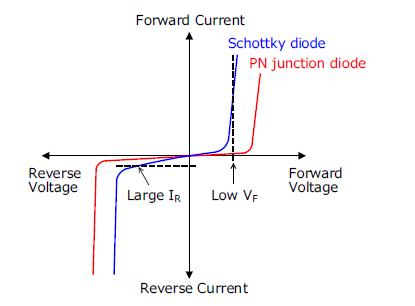
\includegraphics[width=0.5\textwidth]{tech/images/voltage-drop.png}
    \caption{Forward Voltage Drop in Different Diode Types}
    \label{fig:forward-voltage_drop}
    % Diagram showing the forward voltage drop across different types of diodes.
\end{figure}

\subsubsection*{Current Flow in a Diode}
As mentioned earlier, diodes allow current to flow in only one direction. This is due to the PN junction inside the diode, which creates a barrier that prevents current from flowing in the reverse direction. When you apply a forward voltage, this barrier is reduced, and current can flow. Think of it like a gate that only opens one way—pretty neat, right?

\begin{figure}[h]
    \centering
    \begin{circuitikz}
        % First circuit - Forward bias
        \draw (0,0) node[left] {+} 
            to[battery] (0,-2) node[left] {-};
        \draw (0,0) -- (2,0);
        \draw (2,-2) -- (0,-2);
        \draw (2,0) to[D] (2,-2);
        
        % Current flow arrow
        \draw[->, thick, blue] (1,0.3) -- (3,0.3) 
            node[midway, above] {Current flows};
        
        % Label
        \node[below] at (2,-2.5) {Forward Bias};

        % Second circuit - Reverse bias (shifted right)
        \begin{scope}[xshift=6cm]
            \draw (0,0) node[left] {-} 
                to[battery2] (0,-2) node[left] {+};
            \draw (0,0) -- (2,0);
            \draw (2,-2) -- (0,-2);
            \draw (2,0) to[D] (2,-2);
            
            % No current flow symbol (red X)
            \draw[red, thick] (1.7,0.2) -- (2.3,0.5);
            \draw[red, thick] (1.7,0.5) -- (2.3,0.2);
            \node[above] at (2,0.5) {No current};
            
            % Label
            \node[below] at (2,-2.5) {Reverse Bias};
        \end{scope}
    \end{circuitikz}
    \caption{Current Flow in a Diode: Forward bias allows current to flow (left), while reverse bias blocks current flow (right)}
    \label{fig:diode_current_flow}
\end{figure}

\subsubsection*{Cathode Marking on a Diode}
Ever wondered how to tell which side of a diode is the cathode? It's usually marked with a stripe on the package. This stripe is your guide to identifying the cathode, so you don't accidentally connect it the wrong way around. It's like the diode's way of saying, "Hey, this end goes here!"

\begin{figure}[th]
    \centering
    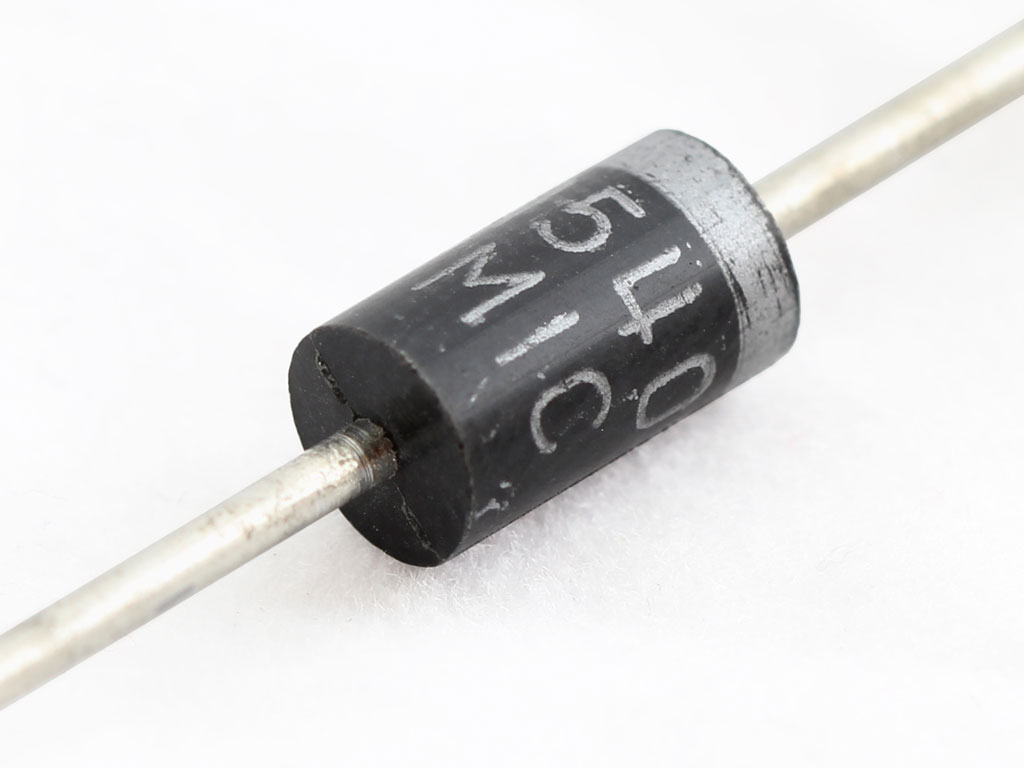
\includegraphics[width=0.3\textwidth]{tech/images/diode.jpeg}
    \caption{Cathode Marking on a Diode: The cathode end is typically identified by a stripe or band around the body of the diode. This marking is crucial for correct installation as diodes must be oriented properly to function. The stripe represents the 'bar' part of the diode symbol, making it easy to correlate the physical component with its schematic representation.}
    \label{fig:cathode_marking}
    % Image showing the marking of the cathode lead on a semiconductor diode.
\end{figure}

\subsubsection*{Light Emission in an LED}
Light-emitting diodes (LEDs) are a special type of diode that emit light when forward current is applied. This happens because the electrons recombine with holes in the semiconductor material, releasing energy in the form of photons. The color of the light depends on the energy gap of the semiconductor material. So, next time you see an LED light up, you'll know it's all about those electrons getting cozy with holes!

\begin{figure}[h]
    \centering
    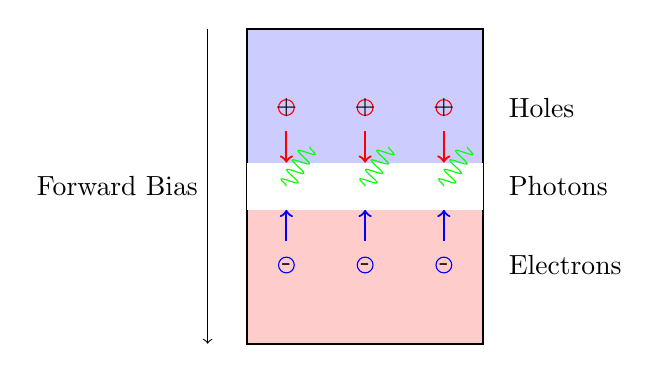
\begin{tikzpicture}
        % P-N Junction structure
        \fill[blue!20] (0,0) rectangle (3,2) node[pos=.5] {P-type};
        \fill[red!20] (0,-2) rectangle (3,0) node[pos=.5] {N-type};
        \draw[black, thick] (0,-2) rectangle (3,2);
        \draw[black, thick] (0,0) -- (3,0);
        
        % Depletion region
        \fill[white!20] (0,-0.3) rectangle (3,0.3);
        
        % Electrons and holes
        \foreach \x in {0.5,1.5,2.5} {
            % Electrons (negative charges)
            \draw[blue] (\x,-1) circle (0.1) node[black] {-};
            \draw[->, blue, thick] (\x,-0.7) -- (\x,-0.3);
            
            % Holes (positive charges)
            \draw[red] (\x,1) circle (0.1) node[black] {+};
            \draw[->, red, thick] (\x,0.7) -- (\x,0.3);
        }
        
        % Light emission
        \foreach \x in {0.5,1.5,2.5} {
            \draw[green, decorate, decoration={snake,amplitude=3pt,segment length=4pt}]
                (\x,0) -- (\x+0.3,0.5);
        }
        
        % Labels
        \node[right] at (3.2,1) {Holes};
        \node[right] at (3.2,-1) {Electrons};
        \node[right] at (3.2,0) {Photons};
        
        % Battery connection
        \draw[->] (-0.5,2) -- (-0.5,-2) node[midway, left] {Forward Bias};
        
    \end{tikzpicture}
    \caption{Light Emission in an LED: When electrons from the N-type material recombine with holes in the P-type material at the junction, energy is released as photons (light)}
    \label{fig:led_light_emission}
\end{figure}

\subsubsection*{Diode Electrodes}
Every diode has two electrodes: the anode and the cathode. The anode is the positive side, and the cathode is the negative side. When you apply a forward voltage, current flows from the anode to the cathode. It's like the diode's way of saying, "This is the way, folks!"

\begin{figure}[h]
    \centering
    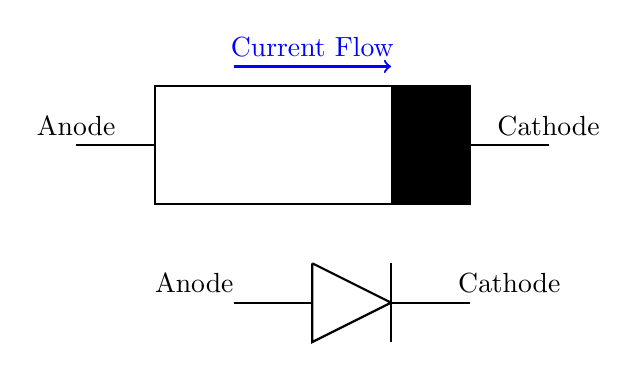
\begin{tikzpicture}
        % Main diode body
        \draw[thick] (0,0) rectangle (4,1.5);
        
        % Leads
        \draw[thick] (-1,0.75) -- (0,0.75);
        \draw[thick] (4,0.75) -- (5,0.75);
        
        % Cathode stripe
        \fill[black] (3,0) rectangle (4,1.5);
        
        % Labels
        \node[above] at (-1.0,0.75) {Anode};
        \node[above] at (5.0,0.75) {Cathode};
        
        % Circuit symbol below
        \begin{scope}[yshift=-2cm]
            \draw[thick] (1,0.75) -- (2,0.75);
            \draw[thick] (2,1.25) -- (2,0.25) -- (3,0.75) -- (2,1.25);
            \draw[thick] (3,1.25) -- (3,0.25);
            \draw[thick] (3,0.75) -- (4,0.75);
            
            % Labels for symbol
            \node[above] at (0.5,0.75) {Anode};
            \node[above] at (4.5,0.75) {Cathode};
        \end{scope}
        
        % Add direction arrow
        \draw[->, thick, blue] (1,1.75) -- (3,1.75) 
            node[midway, above] {Current Flow};
    \end{tikzpicture}
    \caption{Diode Electrodes: Physical package (top) showing the cathode stripe marking, and circuit symbol (bottom) with current flow direction}
    \label{fig:diode_electrodes}
\end{figure}

\begin{table}[h]
    \centering
    \caption{Comparison of Forward Voltage Drop in Diode Types}
    \label{tab:forward_voltage_comparison}
    \begin{tabular}{|l|c|}
        \hline
        \textbf{Diode Type} & \textbf{Forward Voltage Drop (V)} \\
        \hline
        Silicon Diode & 0.7 \\
        Schottky Diode & 0.3 \\
        Germanium Diode & 0.3 \\
        LED (Red) & 1.8 \\
        LED (Blue) & 3.3 \\
        \hline
    \end{tabular}
\end{table}

\subsubsection*{Questions}

\begin{tcolorbox}[colback=gray!10!white,colframe=black!75!black,title={T6B01}]
    Which is true about forward voltage drop in a diode?
    \begin{enumerate}[label=\Alph*),noitemsep]
        \item \textbf{It is lower in some diode types than in others}
        \item It is proportional to peak inverse voltage
        \item It indicates that the diode is defective
        \item It has no impact on the voltage delivered to the load
    \end{enumerate}
\end{tcolorbox}
The forward voltage drop varies depending on the diode type, as different materials and constructions lead to different energy barriers. This is why some diodes, like Schottky diodes, have a lower forward voltage drop compared to silicon diodes.

\begin{tcolorbox}[colback=gray!10!white,colframe=black!75!black,title={T6B02}]
    What electronic component allows current to flow in only one direction?
    \begin{enumerate}[label=\Alph*),noitemsep]
        \item Resistor
        \item Fuse
        \item \textbf{Diode}
        \item Driven element
    \end{enumerate}
\end{tcolorbox}
A diode is specifically designed to allow current to flow in only one direction, thanks to its PN junction.

\begin{tcolorbox}[colback=gray!10!white,colframe=black!75!black,title={T6B06}]
    How is the cathode lead of a semiconductor diode often marked on the package?
    \begin{enumerate}[label=\Alph*),noitemsep]
        \item With the word "cathode"
        \item \textbf{With a stripe}
        \item With the letter C
        \item With the letter K
    \end{enumerate}
\end{tcolorbox}
The cathode is typically marked with a stripe on the diode's package, making it easy to identify.

\begin{tcolorbox}[colback=gray!10!white,colframe=black!75!black,title={T6B07}]
    What causes a light-emitting diode (LED) to emit light?
    \begin{enumerate}[label=\Alph*),noitemsep]
        \item \textbf{Forward current}
        \item Reverse current
        \item Capacitively-coupled RF signal
        \item Inductively-coupled RF signal
    \end{enumerate}
\end{tcolorbox}
When forward current is applied to an LED, electrons recombine with holes, releasing energy in the form of photons, which we see as light.

\begin{tcolorbox}[colback=gray!10!white,colframe=black!75!black,title={T6B09}]
    What are the names for the electrodes of a diode?
    \begin{enumerate}[label=\Alph*),noitemsep]
        \item Plus and minus
        \item Source and drain
        \item \textbf{Anode and cathode}
        \item Gate and base
    \end{enumerate}
\end{tcolorbox}
The two electrodes of a diode are called the anode (positive side) and the cathode (negative side). These terms are standard in diode terminology.
